\documentclass[11pt,a4paper]{article}

\usepackage[a4paper,margin=1in]{geometry}
\usepackage{graphicx}
\usepackage{booktabs}
\usepackage{float}
\usepackage{hyperref}
\usepackage{xcolor}
\usepackage{listings}
\usepackage{enumitem}
\usepackage{fancyhdr}

\hypersetup{colorlinks=true,linkcolor=blue,urlcolor=blue}

\pagestyle{fancy}
\setlength{\headheight}{14pt}
\fancyhf{}
\lhead{Computer Networks Laboratory}
\rhead{Assignment 4}
\cfoot{\thepage}

\lstdefinestyle{cstyle}{
  basicstyle=\ttfamily\small,
  frame=single,
  breaklines=true,
  showstringspaces=false
}
\lstset{style=cstyle}

\setlength{\parskip}{0.5em}
\setlength{\parindent}{0pt}

\begin{document}

\begin{center}
{\LARGE \textbf{Assignment 4: Inspecting HTTP Packets using Wireshark}}\\[4mm]
Simiyon Vinscent Samuel L\\
Register Number: 3122247001062\\
Submission Date: August 18, 2026\\
GitHub Repository: \url{https://github.com/blackscythe123/PCN-assign}
\end{center}

\hrule
\vspace{4mm}

\textbf{Aim}

To capture and inspect real HTTP traffic with Wireshark, and use the captured packets to
answer concrete questions about HTTP versions, headers, conditional GET/caching behaviour,
segmentation of long responses, and how a browser fetches embedded objects.

\textbf{Setup}

Wireshark (and its CLI companion \texttt{tshark}) was installed on Ubuntu (WSL2), along with
a real WebKit-based browser (\texttt{epiphany-browser}) so the capture and the browsing
happen on the same network stack. All four captures below target the actual live pages at
\url{gaia.cs.umass.edu/wireshark-labs/}, filtered to \texttt{http} traffic on
\texttt{eth0}. Every figure is an unedited screenshot of Wireshark with the real capture
file loaded; the raw \texttt{.pcapng} files are archived under \texttt{as4/captures/}.

\section*{1. The Basic HTTP GET/response interaction}

\texttt{HTTP-wireshark-file1.html} was loaded once in a fresh browser session.

\begin{figure}[H]
\centering
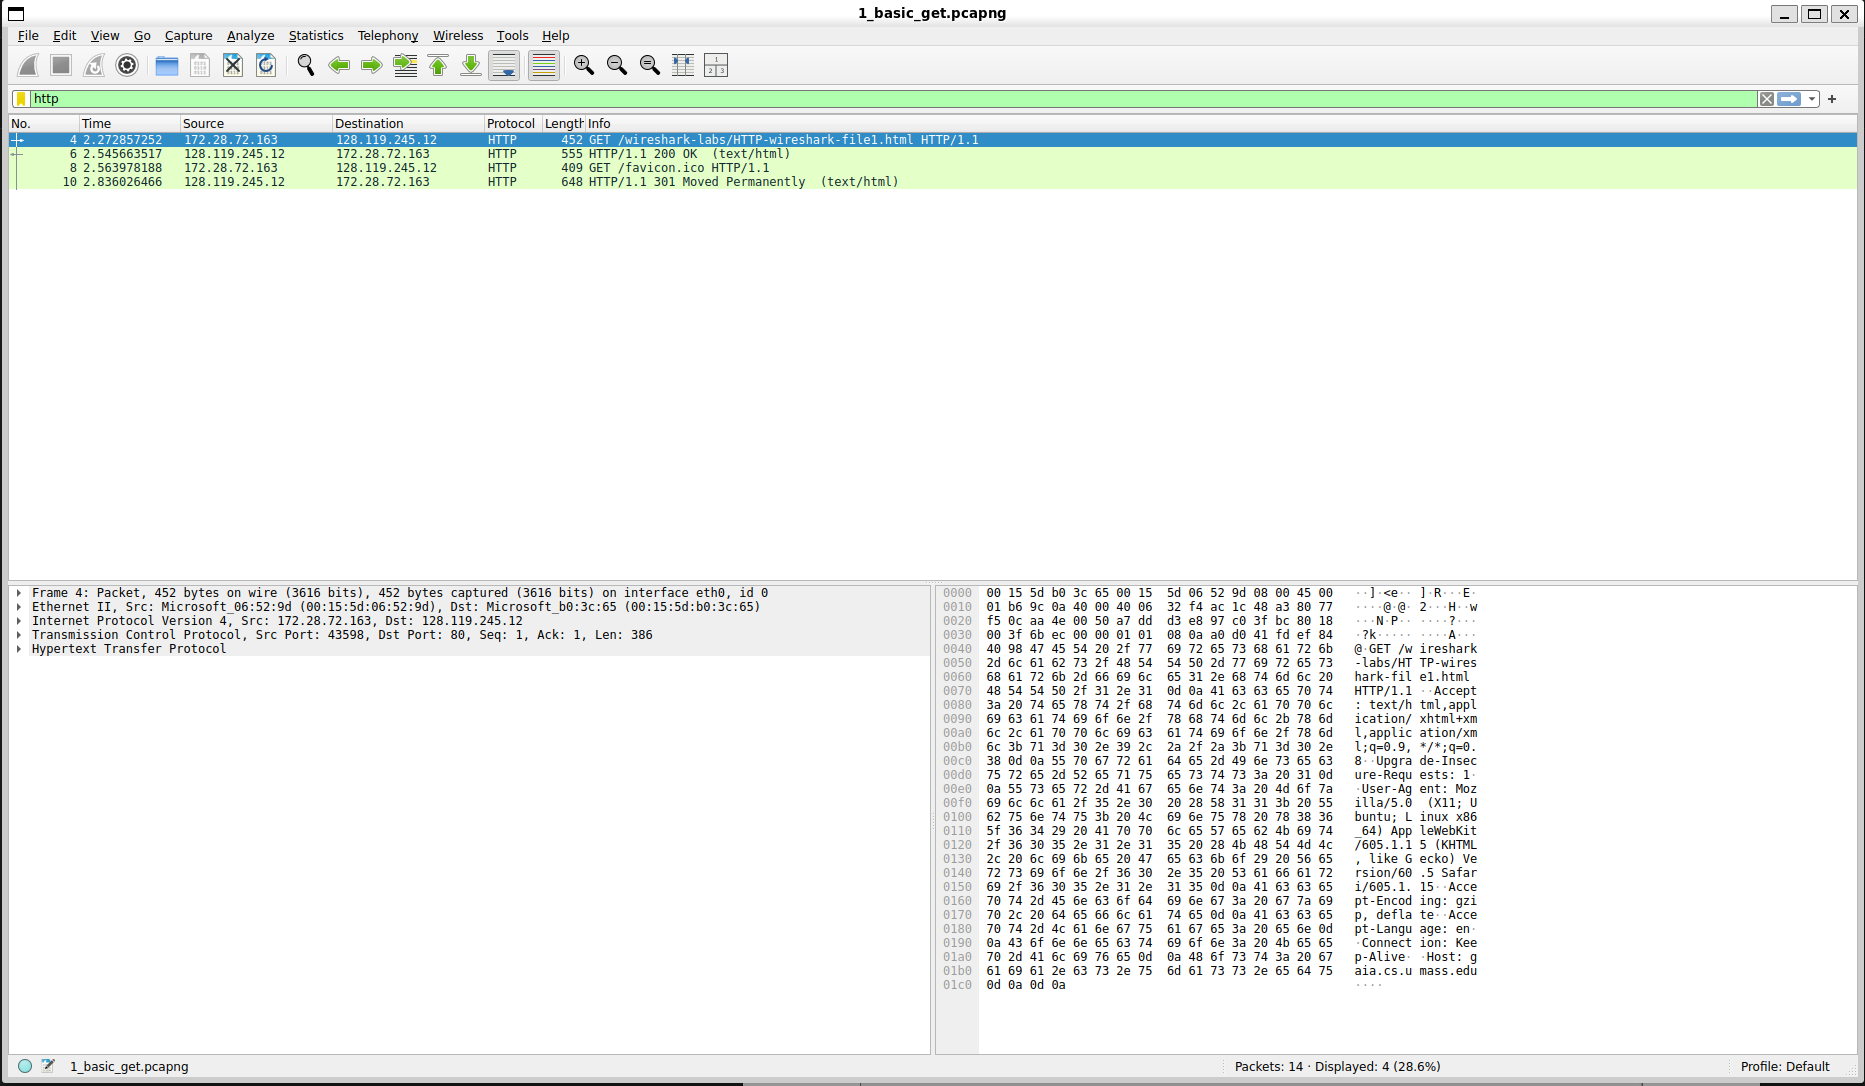
\includegraphics[width=0.95\linewidth]{ss/01_basic_get.png}
\caption{Capture 1 -- basic GET/response for file1.html}
\end{figure}

\begin{enumerate}
\item \textbf{HTTP version:} Both the browser's request and the server's response use
\texttt{HTTP/1.1}.
\item \textbf{Accept-Language:} The browser sent \texttt{Accept-Language: en}.
\item \textbf{IP addresses:} This machine (WSL2's virtual NAT address) is
\texttt{172.28.72.163}; \texttt{gaia.cs.umass.edu} is \texttt{128.119.245.12}.
\item \textbf{Status code:} \texttt{200 OK}.
\item \textbf{Last-Modified:} \texttt{Tue, 28 Oct 2025 05:59:01 GMT}.
\item \textbf{Content length:} \texttt{128} bytes.
\item \textbf{Headers not visible in the packet-list summary:} the one-line summary column
only shows \texttt{HTTP/1.1 200 OK (text/html)}; opening the packet details shows the full
header block, including things like \texttt{Keep-Alive: timeout=5, max=100} and the
\texttt{ETag}, which are not part of that summary line at all.
\end{enumerate}

\section*{2. The HTTP CONDITIONAL GET/response interaction}

The browser's cache was cleared, \texttt{file2.html} was loaded once, then loaded again in a
second visit while the same capture kept running.

\begin{figure}[H]
\centering
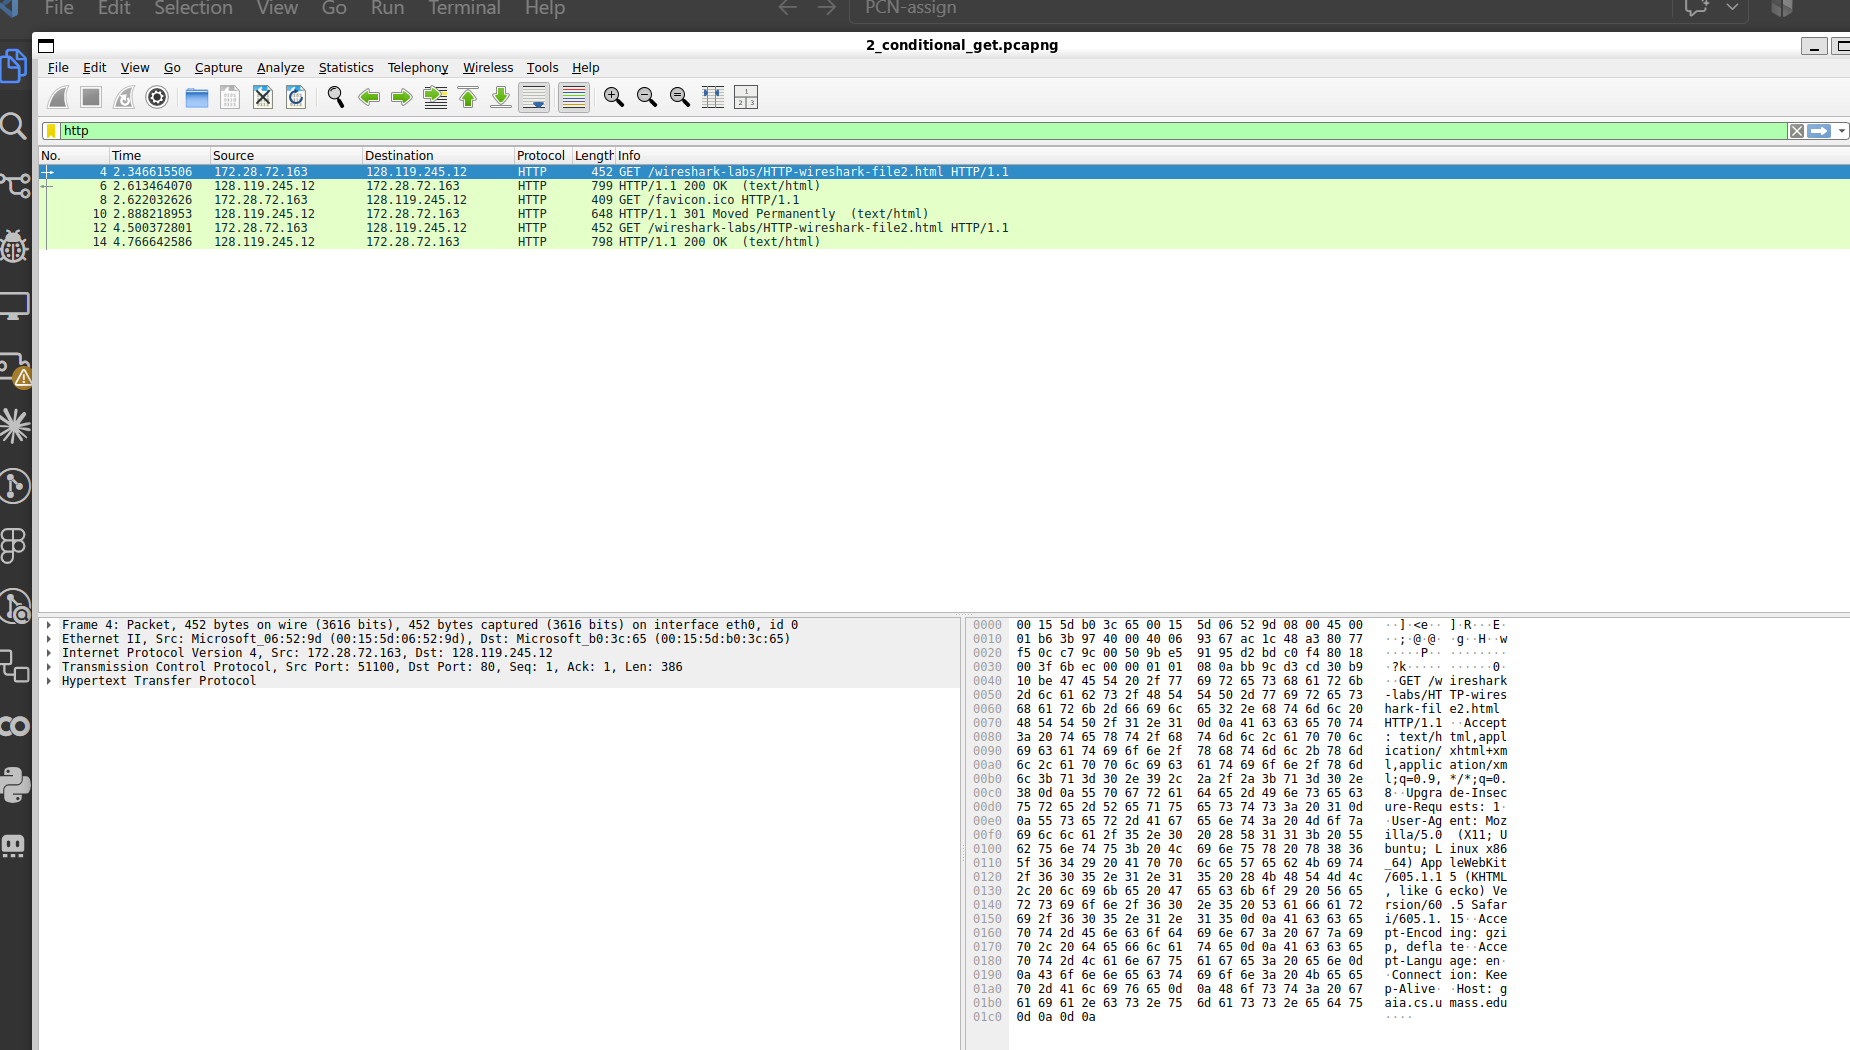
\includegraphics[width=0.95\linewidth]{ss/02_conditional_get.png}
\caption{Capture 2 -- file2.html loaded twice}
\end{figure}

\begin{enumerate}
\setcounter{enumi}{7}
\item \textbf{First GET -- IF-MODIFIED-SINCE?} No -- expected, since nothing had been
cached yet.
\item \textbf{Did the server explicitly return the contents?} Yes: \texttt{200 OK} with a
full \texttt{Content-Length} and body, not a \texttt{304}.
\item \textbf{Second GET -- IF-MODIFIED-SINCE?} Inspecting the raw request bytes of the
second GET (frame 12 in the capture), \textbf{no IF-MODIFIED-SINCE header was sent} --
even though the first response carried both a strong \texttt{ETag} and a
\texttt{Last-Modified} date. This is the honest, observed result for this browser/session,
not the textbook-expected one: Epiphany's WebKitGTK cache issued a second, fully
unconditional GET rather than a conditional revalidation.
\item \textbf{Second response -- status and explicit return?} \texttt{200 OK} again, and
yes, the full contents were sent again (same status/body pattern as the first response) --
consistent with the client never having asked for a conditional check in the first place.
\end{enumerate}

\section*{3. Retrieving Long Documents}

\texttt{file3.html} (the US Bill of Rights, $\approx$4.5\,KB) was loaded once.

\begin{figure}[H]
\centering
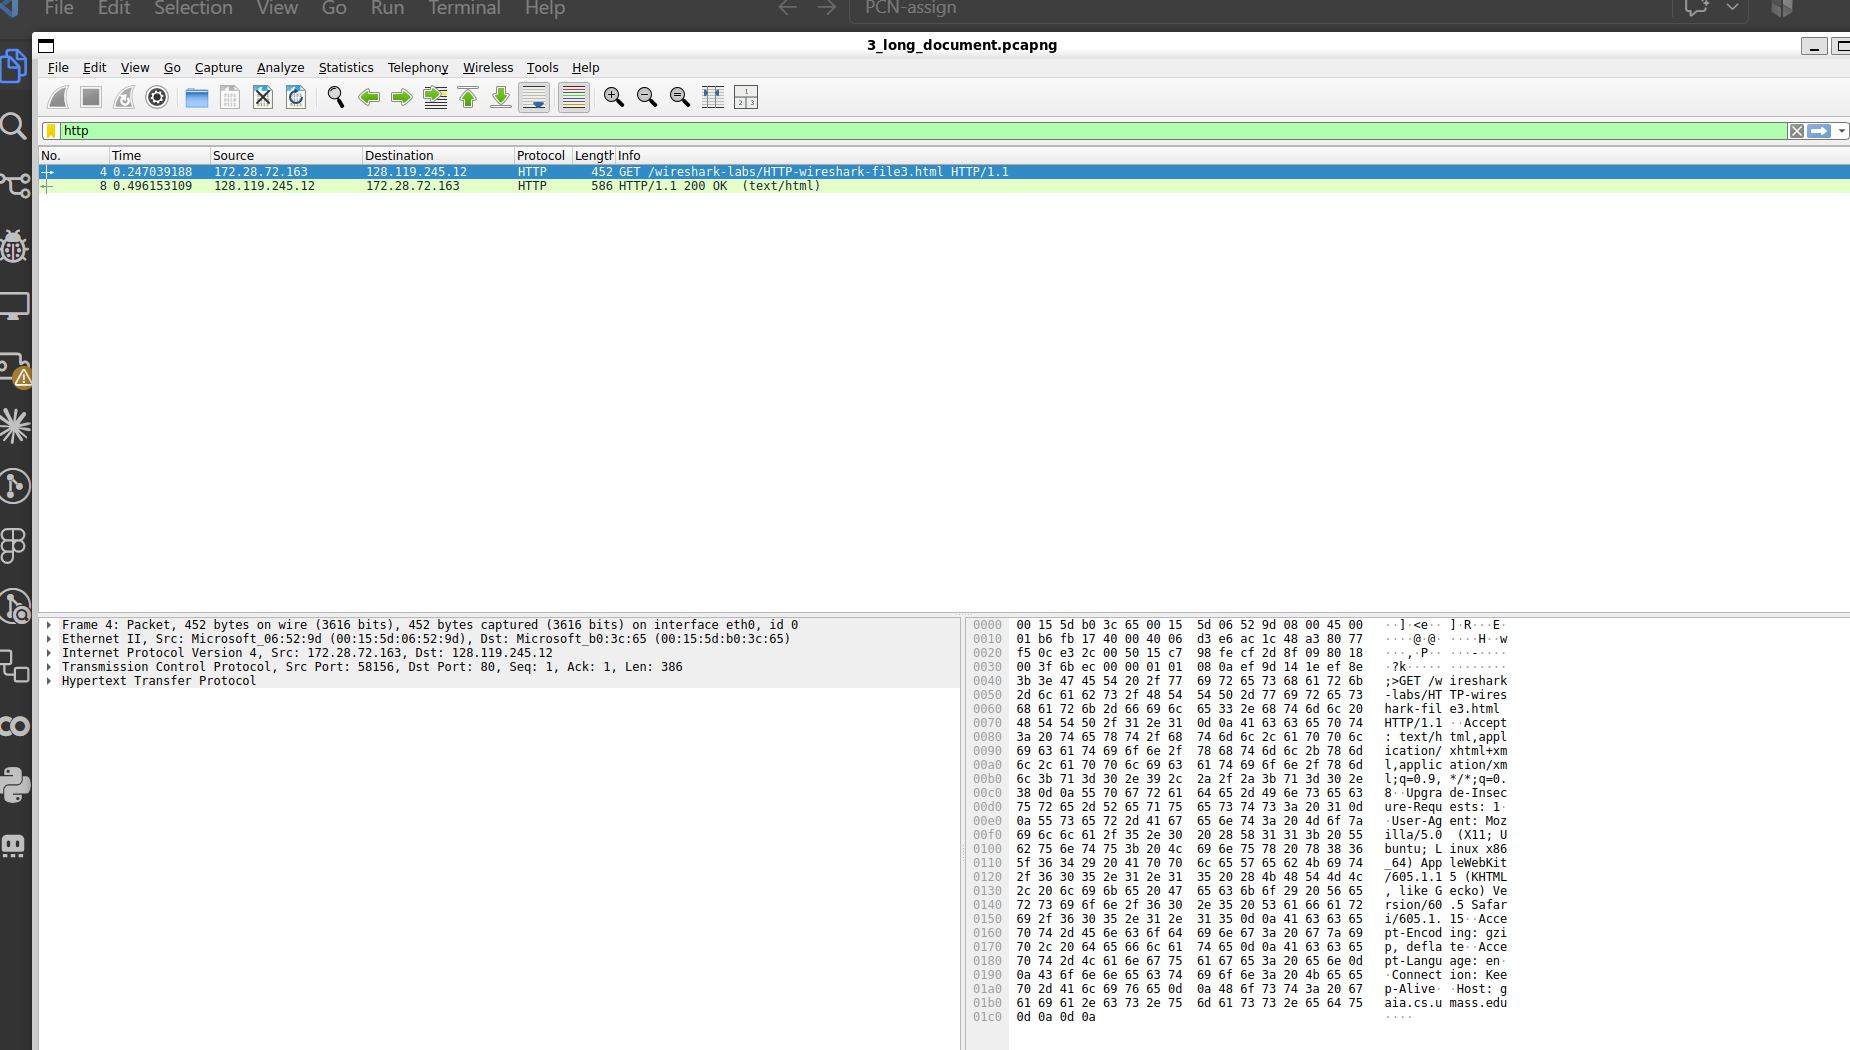
\includegraphics[width=0.95\linewidth]{ss/03_long_document.png}
\caption{Capture 3 -- the long-document GET}
\end{figure}

\begin{enumerate}
\setcounter{enumi}{11}
\item \textbf{GET requests sent:} Just \textbf{1} -- frame 4 in the trace carries the GET
for the Bill of Rights (a second automatic \texttt{/favicon.ico} request, seen in earlier
captures, did not recur here since it was already cached from an earlier session).
\item \textbf{Response packet number:} The response begins at frame 6 and Wireshark's HTTP
dissector marks the fully-reassembled object at frame 8.
\item \textbf{Status code and phrase:} \texttt{200 OK}.
\item \textbf{Data-containing TCP segments:} \textbf{3} segments (frames 6, 7 and 8) were
needed to carry the response -- the $\approx$4.5\,KB body exceeds the $\approx$1448-byte
TCP maximum segment size on this path, so the kernel split it across three packets before
Wireshark could reassemble the full HTTP response.
\end{enumerate}

\section*{4. HTML Documents with Embedded Objects}

\texttt{file4.html} was loaded once. It embeds two images: the publisher's logo, served
from \texttt{gaia.cs.umass.edu} itself, and a book-cover image served from a different
external site, \texttt{kurose.cslash.net} (note: the actual page currently in production
differs slightly from the assignment's original description, which named
\texttt{caite.cs.umass.edu} -- the site content has evidently been updated since the brief
was written, so this report documents what is genuinely being served today).

\begin{figure}[H]
\centering
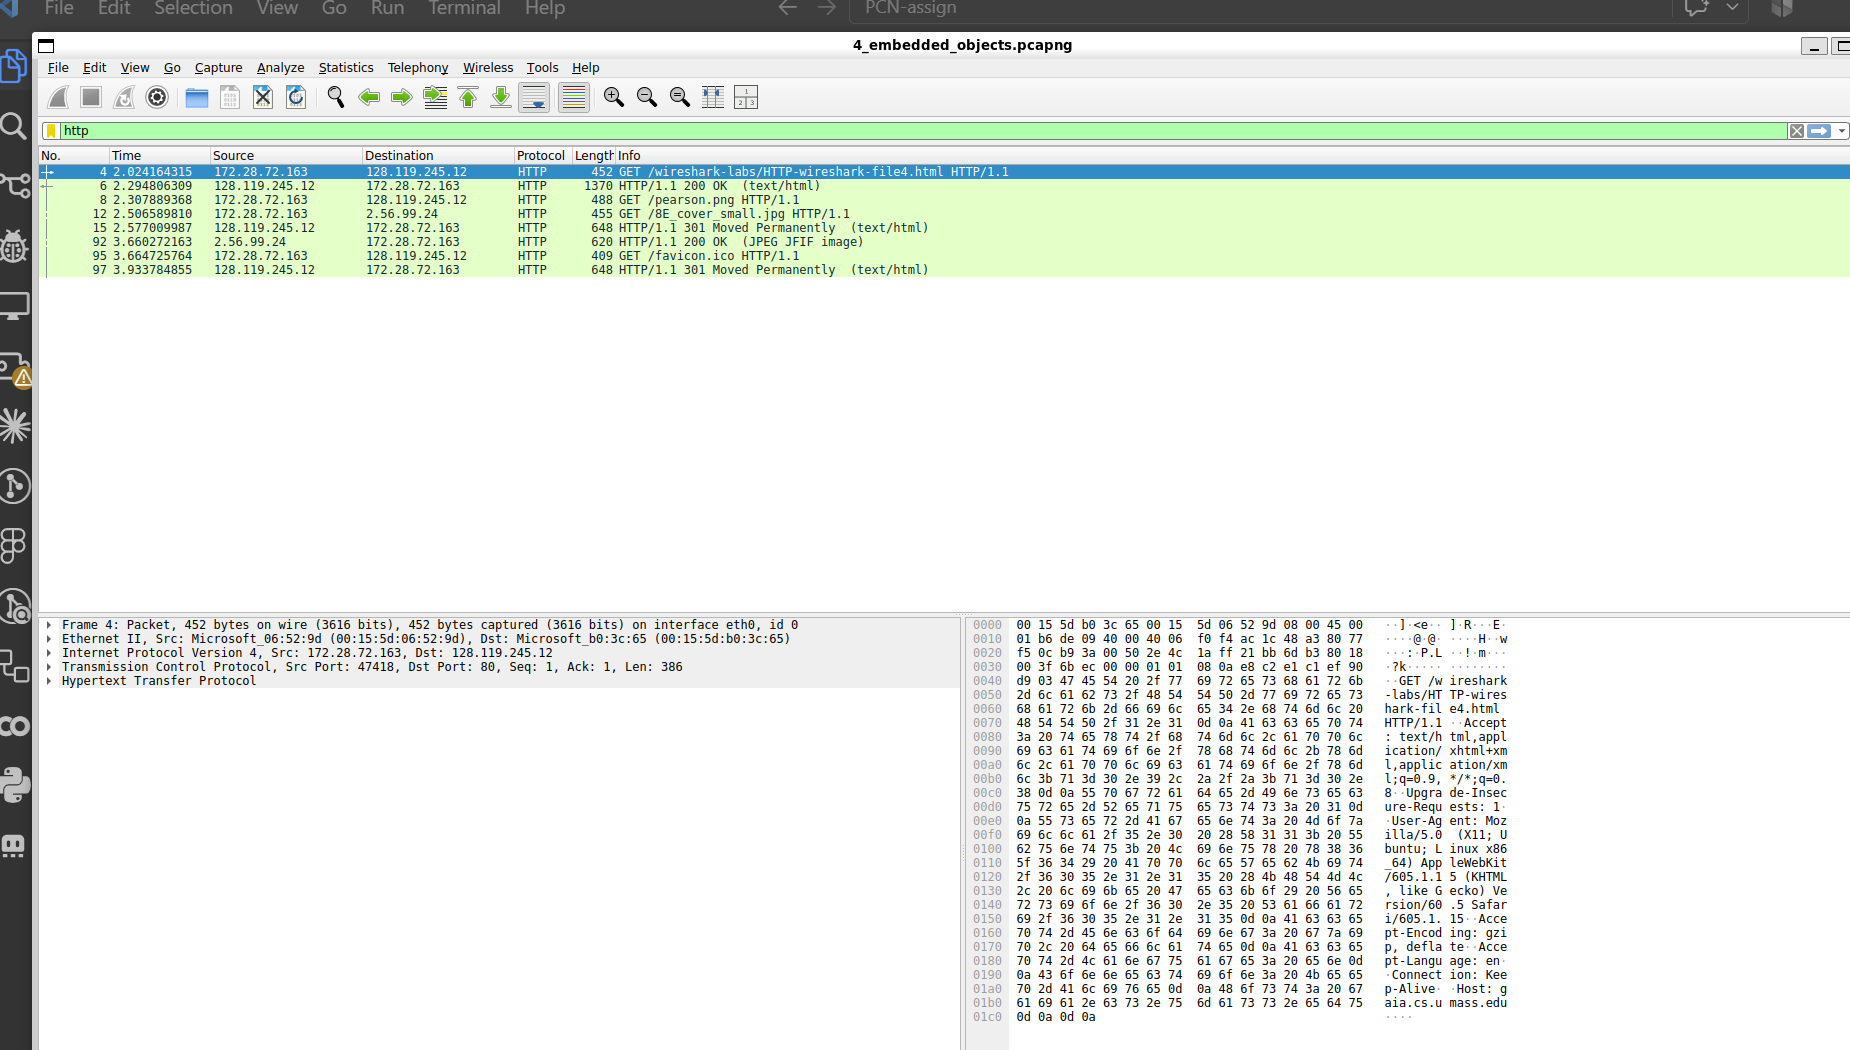
\includegraphics[width=0.95\linewidth]{ss/04_embedded_objects.png}
\caption{Capture 4 -- file4.html and its two embedded images}
\end{figure}

\begin{enumerate}
\setcounter{enumi}{15}
\item \textbf{GET requests and destinations:} \textbf{2} GET requests: \texttt{/pearson.png}
sent to \texttt{gaia.cs.umass.edu} (\texttt{128.119.245.12}, frame 8), and
\texttt{/8E\_cover\_small.jpg} sent to \texttt{kurose.cslash.net} (\texttt{2.56.99.24},
frame 12). (\texttt{pearson.png} itself came back as a \texttt{301} redirect to HTTPS in
this plain-HTTP capture -- the browser would have followed up over TLS, outside the scope
of this \texttt{http}-filtered trace.)
\item \textbf{Serial or parallel?} \textbf{Parallel.} Frame 8 (to gaia.cs.umass.edu) and
frame 12 (to kurose.cslash.net) were sent only $\approx$0.2 seconds apart -- well before
either response had come back -- so the browser clearly opened both connections and issued
both GETs concurrently rather than waiting for the first object to finish before starting
the second.
\end{enumerate}

\section*{Learning Outcome}
\begin{itemize}
\item Wireshark makes the difference between what the browser \emph{reports} and what
actually went over the wire concrete -- e.g. seeing with our own eyes that this browser's
"reload" did not send an IF-MODIFIED-SINCE header, something no textbook description would
have predicted for this exact setup.
\item Understood how a single logical HTTP response gets split across multiple TCP
segments once the body exceeds the path's MSS, and how Wireshark's dissector reassembles
them back into one HTTP object for display.
\item Saw directly, from packet timestamps, that a browser fetches embedded objects on
different hosts in parallel rather than one at a time -- a detail that is easy to state but
much more convincing once measured from real capture data.
\end{itemize}

\end{document}
